\documentclass[border=4pt]{standalone}
\usepackage{fontspec}
\usepackage{amsmath}
\usepackage{unicode-math}
\setmainfont{Latin Modern Roman}
\setmathfont{Latin Modern Math}
\usepackage{pgfplots}
\usepackage{pgfplotstable}
\pgfplotsset{compat=1.18}
\usepackage{tkz-euclide}
\usetikzlibrary{arrows.meta,calc,angles,quotes,patterns,3d,backgrounds}
\definecolor{ink}{HTML}{123428}
\definecolor{asy}{HTML}{475569}
\definecolor{mint}{HTML}{86e0bd}
\tikzset{asym/.style={asy, line width=0.9pt, dash pattern=on 5pt off 3.5pt},
         guide/.style={gray!70, line width=0.6pt, densely dotted},
         dot/.style={circle, inner sep=0pt, minimum size=5pt, draw=white, line width=0.5pt},
         odot/.style={circle, inner sep=0pt, minimum size=5.5pt, fill=white, line width=1pt},
         lab/.style={font=\footnotesize, inner sep=1.5pt, text=ink}}
\begin{document}
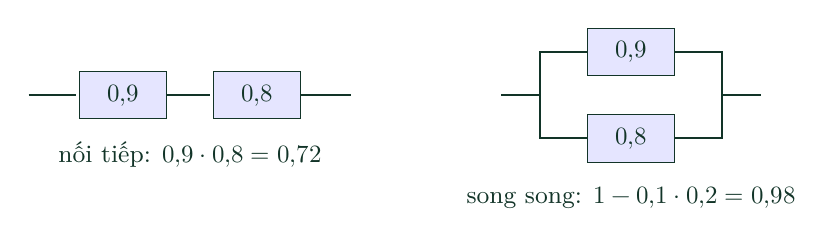
\begin{tikzpicture}[font=\small, every node/.style={text=ink}, box/.style={draw=ink, fill=blue!10, minimum width=1.1cm, minimum height=0.6cm}]
\draw[ink, line width=0.7pt] (0,0) -- (0.6,0); \node[box] (a) at (1.2,0) {$0{,}9$}; \draw[ink, line width=0.7pt] (a.east) -- (2.3,0); \node[box] (b) at (2.9,0) {$0{,}8$}; \draw[ink, line width=0.7pt] (b.east) -- (4.1,0);
\node at (2.05,-0.75) {nối tiếp: $0{,}9\cdot0{,}8=0{,}72$};
\begin{scope}[shift={(6,0)}]
\draw[ink, line width=0.7pt] (0,0) -- (0.5,0) -- (0.5,0.55) -- (1.1,0.55) (0.5,0) -- (0.5,-0.55) -- (1.1,-0.55);
\node[box] (c) at (1.65,0.55) {$0{,}9$}; \node[box] (d) at (1.65,-0.55) {$0{,}8$};
\draw[ink, line width=0.7pt] (c.east) -- (2.8,0.55) -- (2.8,-0.55) -- (d.east) (2.8,0) -- (3.3,0);
\node at (1.65,-1.3) {song song: $1-0{,}1\cdot0{,}2=0{,}98$};
\end{scope}
\end{tikzpicture}
\end{document}
